\documentclass[a4paper]{article}

\usepackage{amsmath, graphicx, float, blindtext} % for dummy text
\graphicspath{ {./images/} }
\title{Overview of the Generalized Linear Model}
\author{Shubham Gupta}

\begin{document}
\maketitle
\section{Introduction}
\begin{itemize}
    \item We will apply the concepts of Bayesian analysis(inference, MCMC, etc) to a more complex family of models called \textbf{generalized linear models} which consists of models such as t-tests, analysis of variance(ANOVA). multiple regression, logistic regression, log-linear models, etc.
\end{itemize}
\section{Types of Variables}
\begin{itemize}
    \item Two main types of variables: \textbf{Predictor} and \textbf{Predicted} variables.  
    \item Likelihood functionn expresses probability of values for the \textbf{predicted} variable as a function of values of the \textbf{predictor} variable.  
    \item Predictor variables are called \textbf{depdendant} variables.
    \item Predicted variables are called \textbf{independant} variables. 
\end{itemize}
\subsection{Scale types}
\begin{itemize}
    \item Main types are:
        \begin{itemize}
            \item Metric
            \item Ordinal
            \item Nominal
            \item Count
        \end{itemize}
\end{itemize}
\section{Linear combination of predictors}
\begin{itemize}
    \item GLM expresses influence of predictors as their \textbf{weighted sum}.  
\end{itemize}
\subsection{Linear function of a single metric predictor}
\begin{itemize}
    \item Linear functions preserver proportinality.
        \[
            y = \beta_0 + \beta_1x
        .\] 
    \item This type of equation is called an \textbf{affine}. 
\end{itemize}
\subsection{Additive combination of metric predictors}
\begin{itemize}
    \item Add predictor variables for combined effect. 
        \[
            y = \beta_0 + \sum_{k=1}^{K} \beta_kx_k
        .\] 
\end{itemize}
\subsection{Non additive interaction of metric predictors}
\begin{itemize}
    \item Even if the interactions between two predictors are \textbf{not linear}, a new feature(like their product or sum) can help make the dataset linear. 
\end{itemize}
\subsection{Nominal Predictors}
\subsubsection{Linear model for a single nominal predictor}
\begin{itemize}
    \item Also called as \textbf{one hot encoding}. Split the nomial variables into multiple columns to model the problem. 
        \[
            y = \beta_0 + \beta_{[1]}x_{[1]} + \beta_{[2]}x_{[2]} + \ldots  
        .\] 
        \[
            y = \beta_0 + \vec{\beta} . \vec{x} 
        .\] 
\end{itemize}
\subsubsection{Additive combination of nominal predictors}
\begin{itemize}
    \item Effect of multiple nominal predictors combinations can be represented by:
        \[
            y = \beta_0 + \sum_{n}\beta_{1[j]}x_{1[j]} + \sum_{n}\beta_{2[k]}x_{2[k]} + \ldots
        .\] 
\end{itemize}
\subsubsection{Nonadditive interaction of nominal predictors}
\begin{itemize}
    \item $\vec{x}_{1x2}$ refers to a particular combination of values from $\vec{x_1}$ and $\vec{x_2}$.
    \item Nonadditive interaction is represented by:
        \[
            y = \beta_0 + \beta_{[1]}x_{[1]} + \beta_{[2]}x_{[2]} + \vec{\beta_{1x2}} . \vec{x_{1x2}} 
        .\] 
        \begin{figure}[H]
            \centering
            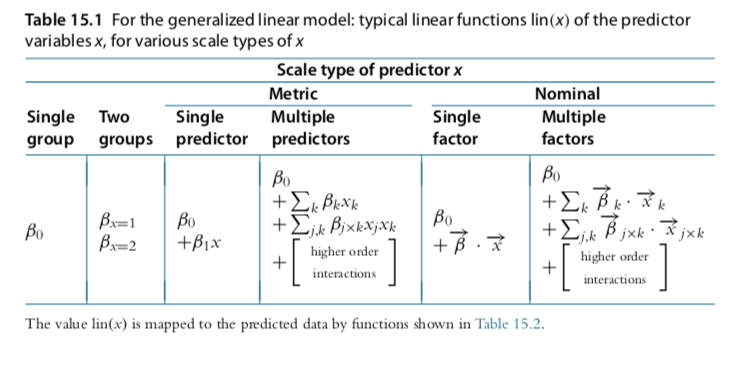
\includegraphics[width=0.8\textwidth]{linear_functions}
            \caption{Typical linear functions}
            \label{fig:linear_functions}
        \end{figure}
\end{itemize}
\subsection{Linking from combined predictors to noisy predicted data}
\subsubsection{From predictors to predicted central tendency}
\begin{itemize}
    \item Preditor variables need to be mapped to predicted variable. This is called \textbf{(inverse) link function}.
        \[
            y = f(lin(x))
        .\] 
    \item $f$ is also called \textbf{mean} function as it generally represents the central measure of the data. 
\end{itemize}
\subsubsection{Logistic function}
\begin{itemize}
    \item Logistic function can be written as:
        \[
            y = \frac{1}{1+\exp^{-x}} 
        .\] 
    \item The value ranges between 0 and 1.
    \item It can be expressed with gain $\gamma$ and threshold $\theta$.
        \begin{itemize}
            \item $\theta$ Point on x-axis for which $y=0.5 $.
            \item $\gamma$ indicates how steeply logistic function rises through a point.
        \end{itemize}
        \[
            y = logistic(x;y,\theta) = \frac{1}{1+\exp(-y(x-\theta))}
        .\] 
        \begin{figure}[H]
            \centering
            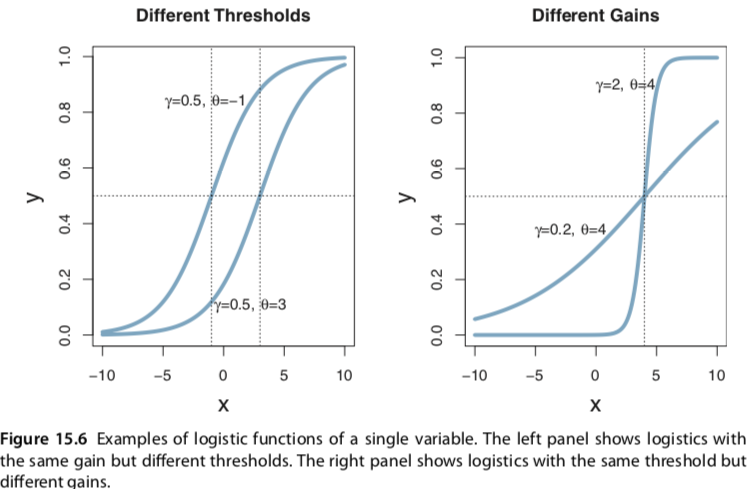
\includegraphics[width=0.8\textwidth]{logistic_function}
            \caption{Threshold and Gain values for logistic function}
            \label{fig:logistic_function}
        \end{figure}
    \item For logistic function with multiple variables, we will use the normalized form:
        \[
            y = logistic(y \sum_{k} w_kx_k-\theta))
        .\] 
    \item It also has the following condition:
        \[
            (\sum_{k} w_k^2)^\frac{1}{2} = 1
        .\] 
        \begin{figure}[H]
            \centering
            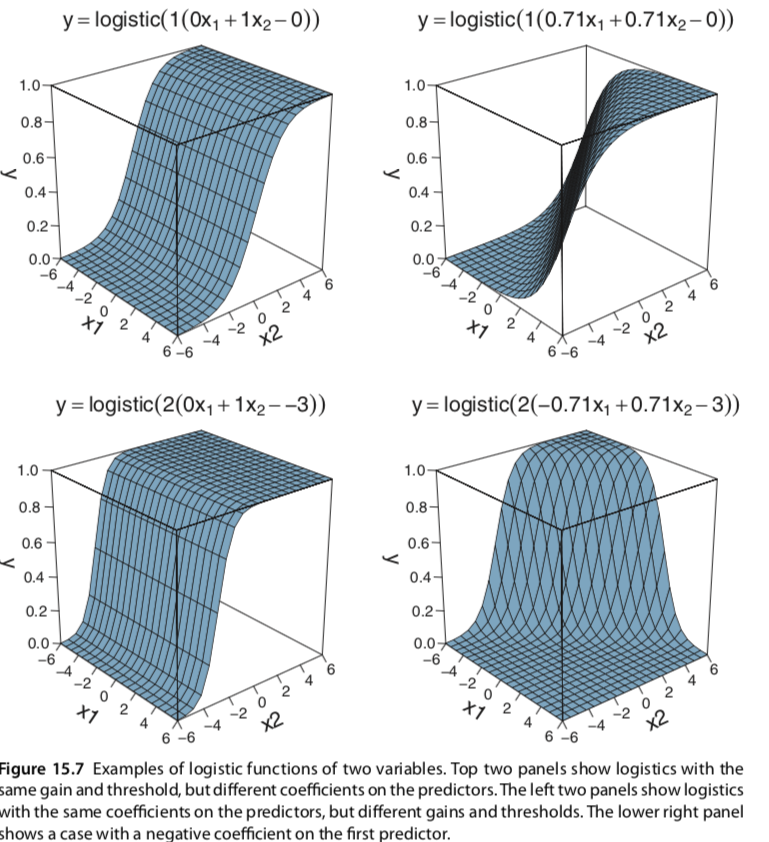
\includegraphics[width=0.8\textwidth]{multi_variable_logistic}
            \caption{Logistic functions of two variables}
            \label{fig:multi_variable_logistic}
        \end{figure}
    \item Coefficients of $x_1$ and $x_2$ determine the \textbf{oritentation} of the cliff. 
    \item Threshold $\theta$ determines the \textbf{position} of the logistical cliff.   
    \item Gain $\gamma$ determines steepness of the logistical cliff.
    \item Inverse of logistic function is called \textbf{logit} function. 
        \[
            \text{For } 0 < p < 1, logit(p) = log([\frac{p}{1-p}])
        .\] 
\end{itemize}
\subsubsection{The cumalative normal function}
\begin{itemize}
    \item Generally used when we can model a variable as continous with normally distributed variability.
    \item Denoted as: $\phi(x; \mu, \sigma)$
    \item $mu$ is similar to threshold($\theta$ ) of logistic function.
    \item $\sigma$ is the inverse of gamma($\gamma$ ) value in logistic function i.e smaller value of $\sigma \implies$ steeper cumalative normal.
    \begin{figure}[H]
        \centering
        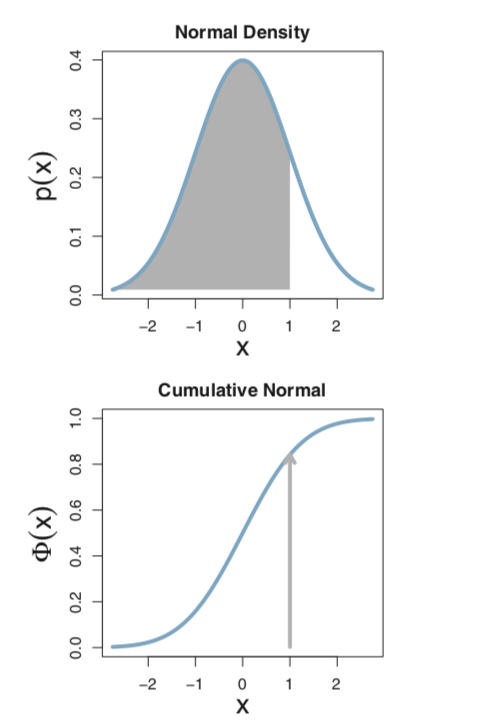
\includegraphics[width=0.8\textwidth]{cumalative_normal}
        \caption{Cumalative normal}
        \label{fig:cumalative_normal}
    \end{figure}
    \item Inverse of cumalative normal is called \textbf{probit} function. Probit maps value between 0.0 and 1.0 
\end{itemize}
\subsection{Predicted central tendency to noisy data}
\begin{itemize}
    \item We can always only predict the \textbf{probability} that y will be equal to some value. Due to this, we do not equate $y = f(lin(x))$ but instead we say it will be  \textbf{near} that value.  
    \item Hence, we use the \textbf{probability density function}. If $\mu$ represents some central tendency(need not always be mean), then we have:
    \[
        y \sim pdf(\mu, [scale, shape, etc.])
    .\] 
    \item \textbf{pdf} is affected by parameters such as scale, shape, etc. 
    \item Typical link functions and pdfs for various predicted variables are:
    \begin{figure}[H]
        \centering
        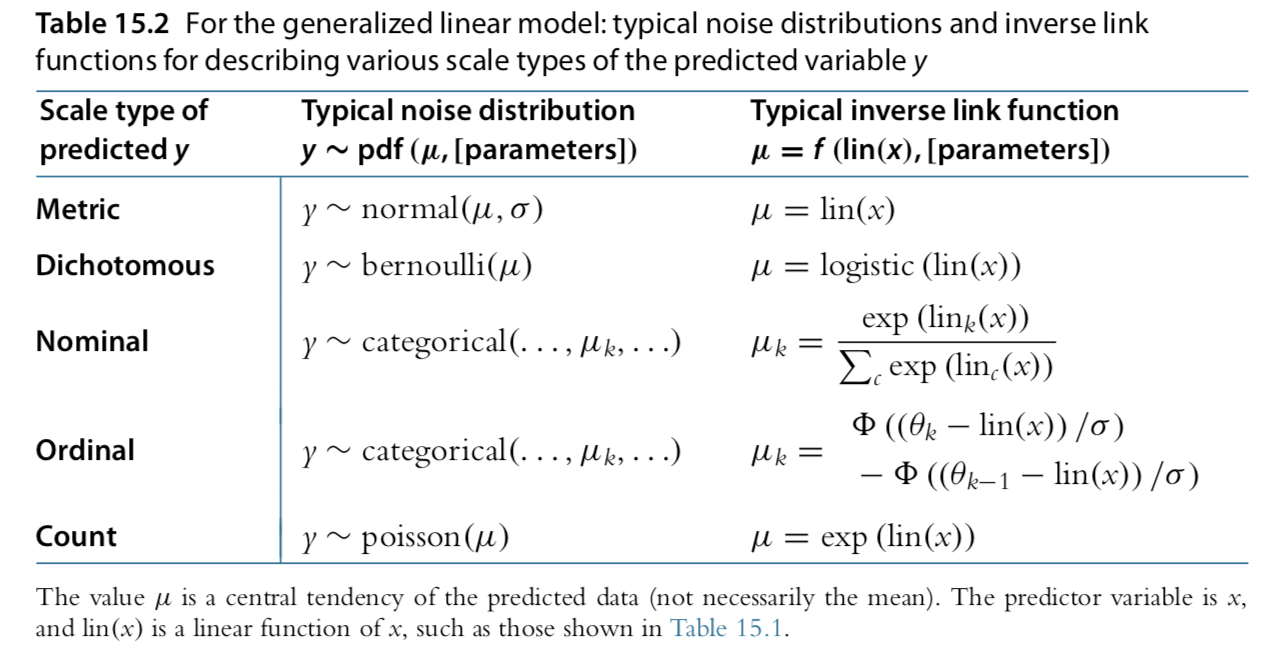
\includegraphics[width=0.8\textwidth]{typical_link_pdf}
        \caption{Link functions and PDF for different y variables}
        \label{fig:typical_link_pdf}
    \end{figure}
\end{itemize}
\subsection{Formal expression of the GLM}
\begin{itemize}
    \item GLM can be written as follows:
    \[
        \mu = f(lin(x), [parameters])
    .\] 
    \[
        y \sim pdf(\mu, [parameters])
    .\] 
\end{itemize}
\subsubsection{Cases of GLM}
\begin{itemize}
    \item The table below tells us how to figure out which data can be predictors and which data cna be predicted:
    \begin{figure}[H]
        \centering
        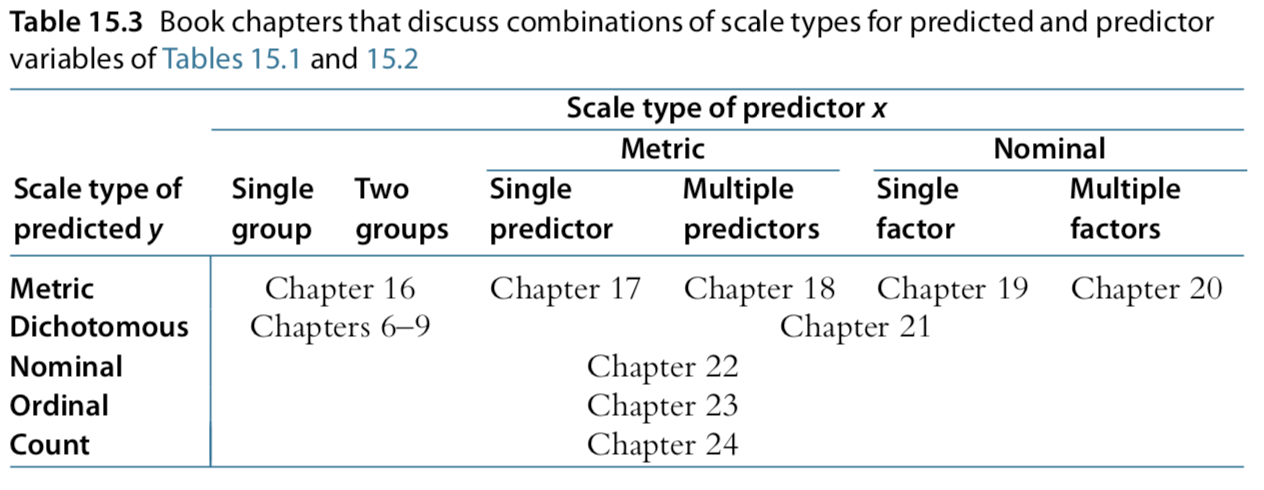
\includegraphics[width=0.8\textwidth]{glm_table}
        \caption{Generic table for GLM}
        \label{fig:glm_table}
    \end{figure}
\end{itemize}
\end{document}
